\chapter{Implementation}

%The implementation should look at any issues you encountered as you tried to implement your design. During the work, you might have found that elements of your design were unnecessary or overly complex; perhaps third party libraries were available that simplified some of the functions that you intended to implement. If things were easier in some areas, then how did you adapt your project to take account of your findings?

%It is more likely that things were more complex than you first thought. In particular, were there any problems or difficulties that you found during implementation that you had to address? Did such problems simply delay you or were they more significant?

%You can conclude this section by reviewing the end of the implementation stage against the planned requirements.

\section{Image processing} \label{imp:image_proces}
The image processing would prove to be an integral part of the application, enhancing the ability to learn handwriting more effectively and efficiently. The end script was implemented over a series of sprints.
\subsection{Optimising tesseract}
After the design considerations to use OpenCV was chosen, specific algorithms would need to be implemented. After a discussion with Dr Hannah Dee, it was suggested that investigations into different binarisation scripts would be useful.

\subsubsection{OTSU}
OTSU, created by Nobuyuki Otsu, is a binarisation technique which essentially converts an image to black and white. Otsu is a global thresholding algorithm, using the whole image as a comparsion. This is unlike local thresholding algorithms where comparisons are made pixel by pixel \cite{citeulike:6044081}.

Due to notes having non-uniform lighting by the intrusion of shadows on an image, this makes OTSU difficult to reliably binarise the image.

\begin{figure}[H]
  \centering
  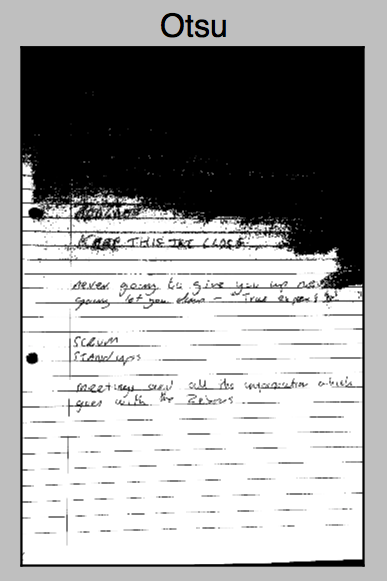
\includegraphics{images/OTSU}
  \label{fig:OTSU}
  \caption{The use of OTSU binarisation technique on an image with a little shadow across the image}
\end{figure}

Figure \ref{fig:OTSU} shows the binarisation technique on an image with the a slight shadow imposed on the image. Clearly it can be seen that it binarises the wrong sections of the image, this would be due to global thresholding.

The basic premise of OTSU is the image's grey-level values are segmented into a series of histograms. OTSU determines the optimial threshold value by ``maximising the discriminant measure'' \cite{citeulike:2917492}. In other words, OTSU attempts to maximise the margin between the histograms. From the maximising of the histograms, pixels can be segmented into their background or foreground pixels \cite{citeulike:14021372}.

HP, who created Tesseract, describe OTSU as its underlying pre-processing algorithm when it tries to identify characters \cite{citeulike:13931186}. From the iterative spike work with OTSU it is clear to see, just from Figure \ref{fig:OTSU}, how Tesseract would be unable to clearly identify characters from that image.

Overall, OTSU, although it is a very solid binarisation method, it suffers from imposed shadows over images. This would not be the best option to choose when choosing an appropriate binarisation technique.

\subsubsection{Adaptive threshold} \label{section:threshold}
From the enlighting analysis of OTSU it was realised that using an OTSU thresholding ontop of an OTSU threshold from the Tesseract engine would not be beneficial. Therefore, in the next iteration of the script, an adaptive threshold approach was chosen.

Adaptive threshold will calculate the threshold over a series of smaller segments of the image \cite{citeulike:14021401}. This reduces the impact of shadows over an image, and does not consider global illumination as the key.

Using the OpenCV library there was two options \cite{citeulike:1402140}:
\begin{enumerate}
  \item Gaussian adaptive threshold which is the weighted sum of the neighborhood
  \item Mean adaptive threshold, which is the mean of neighborhood.
\end{enumerate}

\begin{figure}[H]
  \centering
  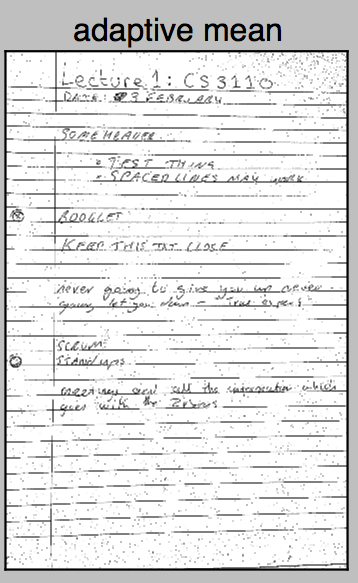
\includegraphics{images/adaptive_mean}
  \caption{Adaptive mean threshold algorithm on a note, showing binarisation but there is still noise in the image.}
  \label{fig:adaptive_mean}
\end{figure}

The mean neighboured takes a block size around the pixel, say 4, and will work out the mean pixel value from that block. The mean value selected will then be selected as the thresholding value, which will determine whether pixels are background or foreground \cite{citeulike:14021401}. Figure \ref{fig:adaptive_mean} shows a mean adaptive threshold. Due to smoothing issues there is still noise on the image.

The gaussian operation differs from the mean as it uses a gaussian value over the sub-image. Firstly each ``blocksize'' is a value which surround the pixel. A default gaussian weight is then calculated [ADD calculation] based on the blocksize. For every pixel in the block, multiply it by the gaussian, an average weight is then taken and used as a threshold \cite{bradski2008learning}\cite{citeulike:1402140}.


\begin{figure}[H]
  \centering
  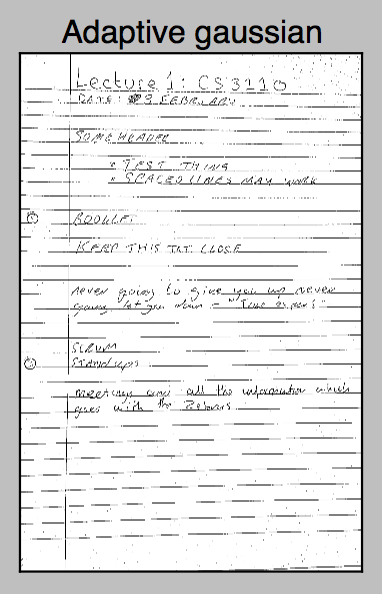
\includegraphics{images/adaptive_gaussian}
  \caption{Adaptive Gaussian used over the image, showing a lot smoother of an image}
  \label{fig:adaptive_gaussian}
\end{figure}

Figure \ref{fig:adaptive_gaussian} shows the adaptive gaussian shows an image which is working it's way to binarisation. It does not have a shadow overlaying the image and the text, lines and little noise have been extracted.

\begin{figure}[H]
  \centering
  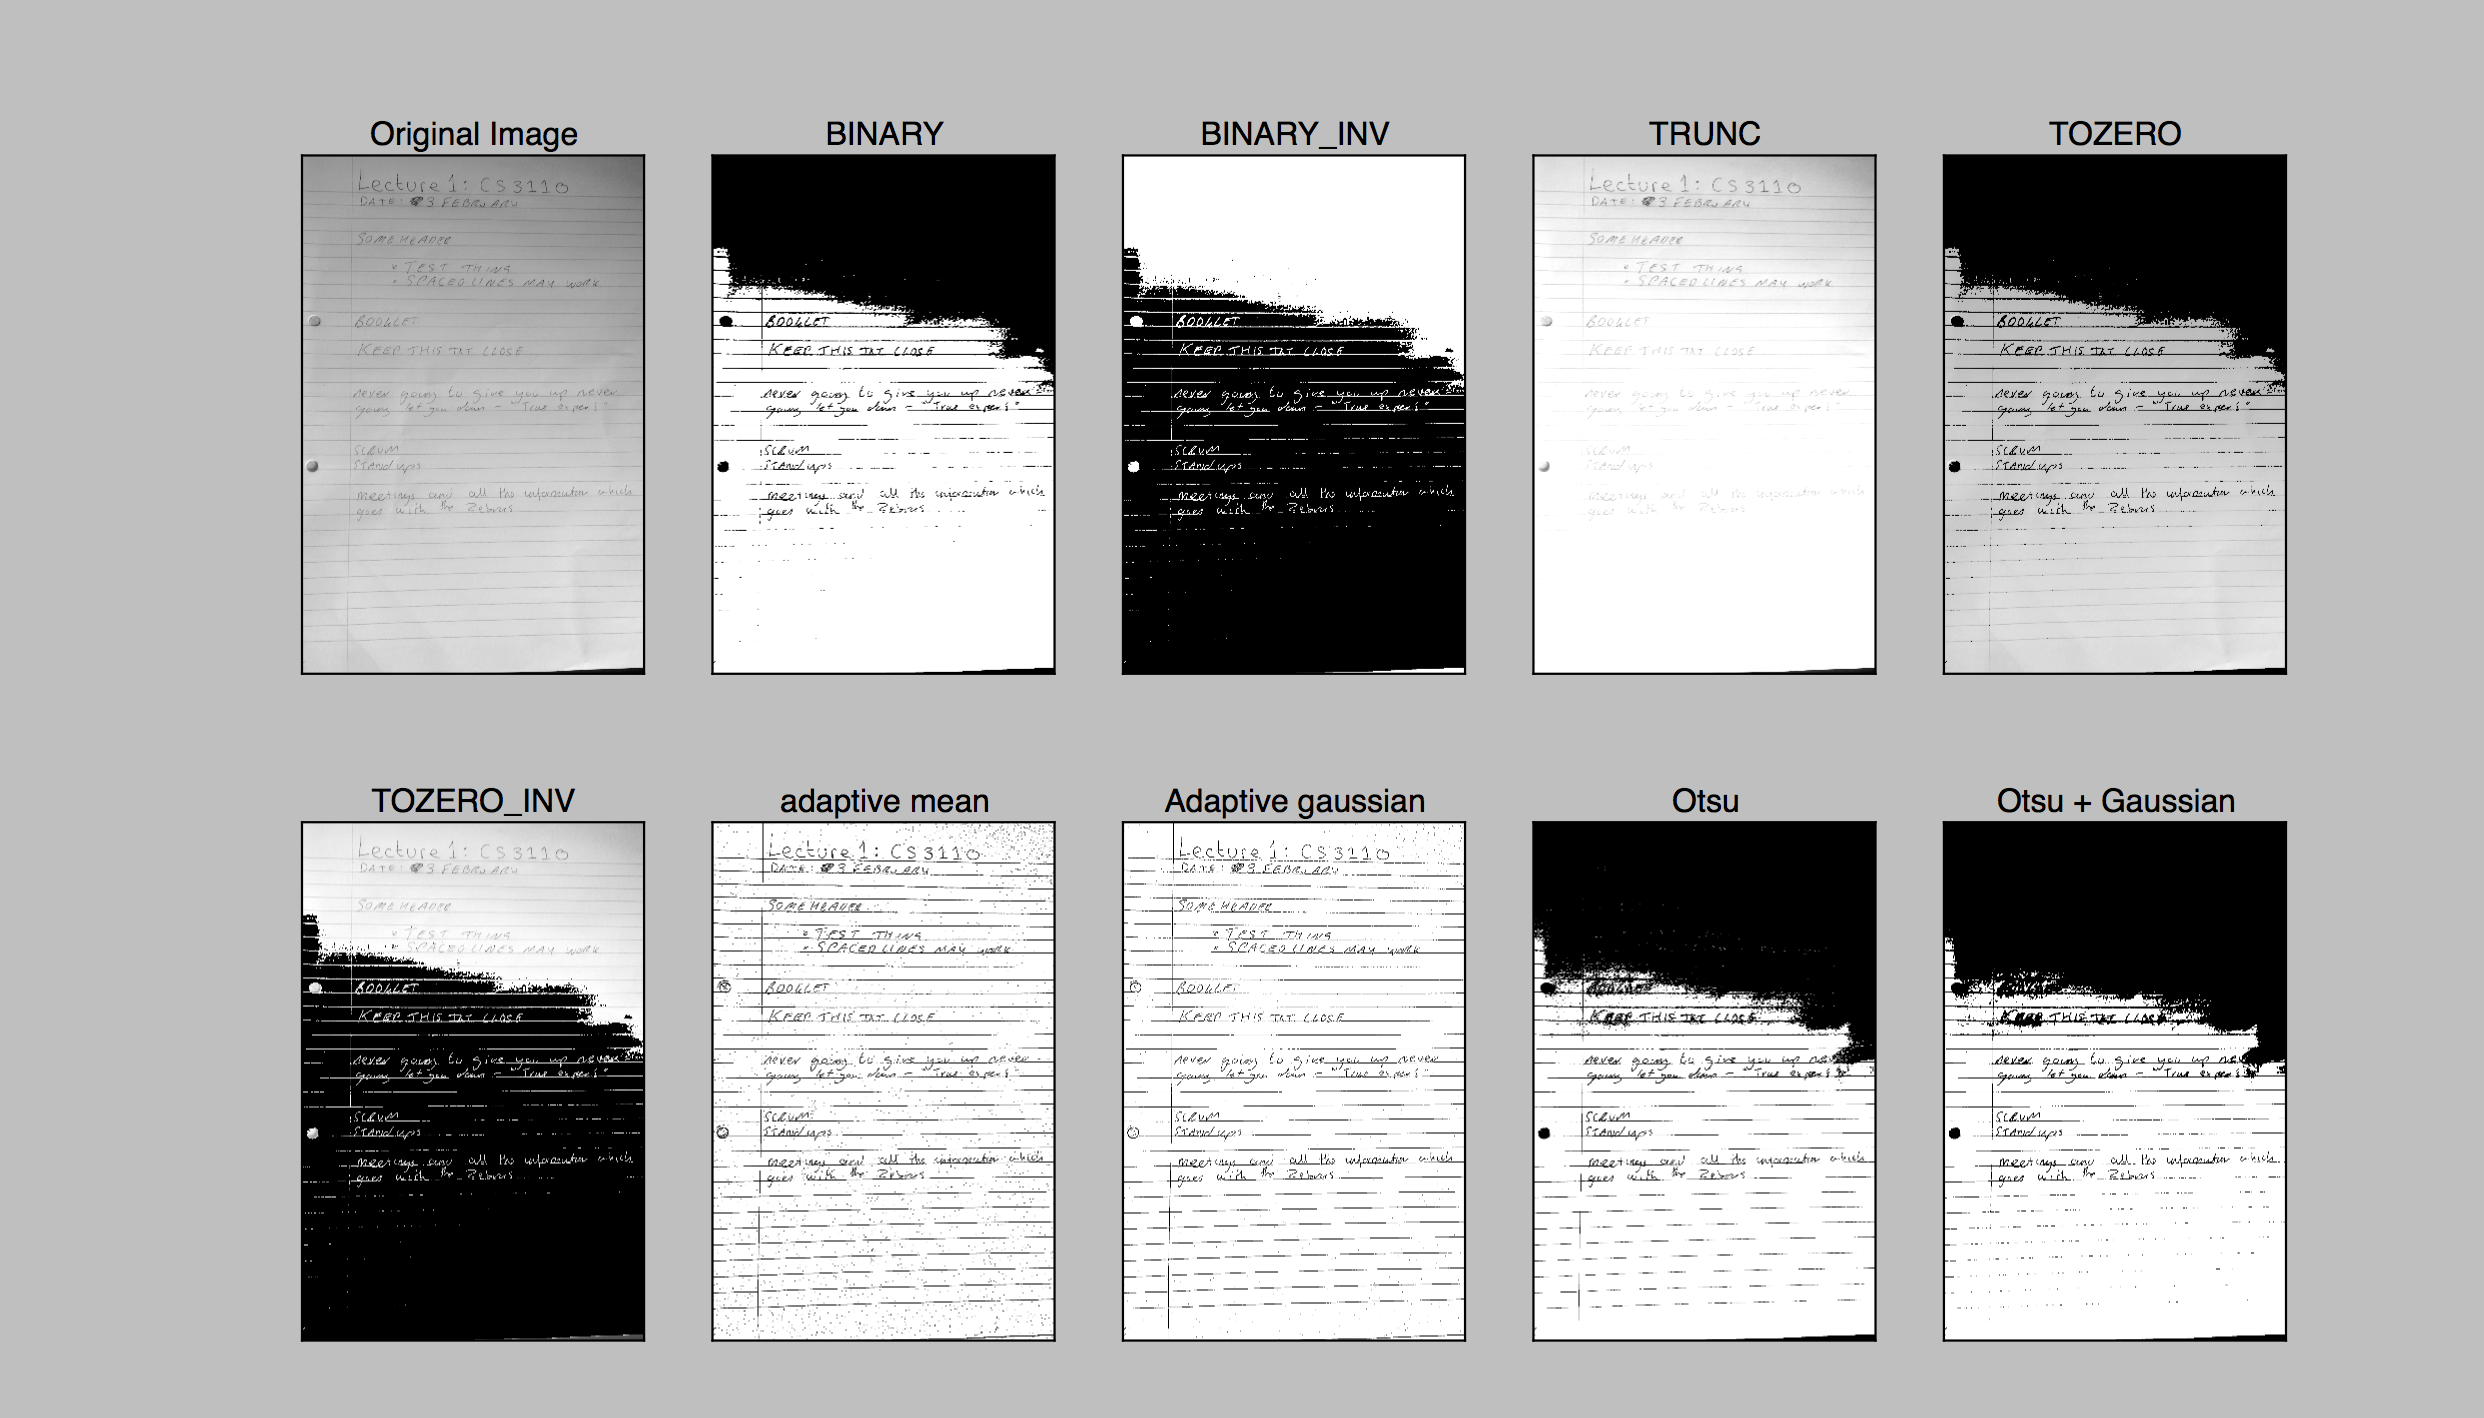
\includegraphics[scale=0.3]{images/thresholding_options}
  \caption{A variety of thresholding techniques used on the same note, showing adaptive threshold resulting in the best}
  \label{fig:thresholding_options}
\end{figure}

Figure \ref{fig:threshold_options} displays the other types of thresholding options iteratively tried. It was decided that the gaussian adaptive thesholding would be implemented and improved with different morphological operations.

\section{Lined paper}
Intially standard lined paper was used for the notes, but the noise produced from the lines was too much to ensure reliable readings from, Tesseract. Refer to appendix \cite{appendix:image_processing} section \cite{processing:pre-line}.

\subsection{Filtering the blue lines}
Custom lined paper, with equal spacing was constructed to overcome this as discussed in section \ref{}.

Over a few iterations the main aim was to remove the blue lines from the image.
\begin{algorithm}
\caption{Initial removing the blue lines algorithm}
\label{algorithm:threshold1}
\begin{algorithmic}[1]
  \Function{remove\_lines}{}
    \State image $\gets$ read\_image\_as\_grayscale()
    \State lower\_black $\gets$ np.array([0,0,0])
    \State upper\_black $\gets$ np.array([175,20, 95])
    \State mask\_black $\gets$ cv2.inRange(erode, lower\_black, upper\_black)
    \State mask[np.where(mask\_black == 0)] $\gets$ 255
  \EndFunction
  \end{algorithmic}
\end{algorithm}

Algorith \ref{algorithm:threshold1} has its obviousy flaws. It attempts to get the values between a grey-black color range. The blue lined tex would obviously have some black content in it, so not all the lines would be removed.

\begin{figure}[H]
  \centering
  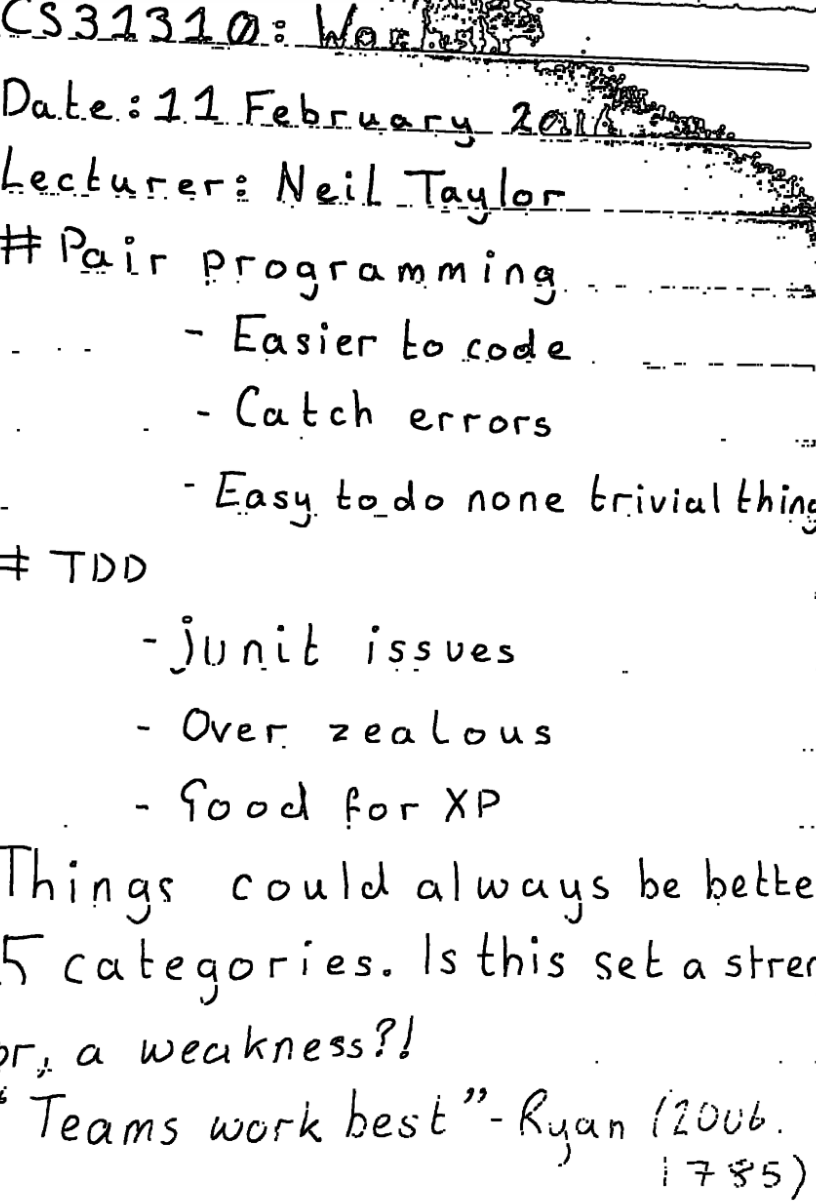
\includegraphics{images/removed_lines_still_noise}
  \caption{An example of the above algorithm. There is still significant amounts of noise in the image.}
  \label{fig:remove_lines_noise}
\end{figure}

After morphological operations such as erroding and dilation, the line noise was no longer being removed and insteadit began to affect the quality of the segmentation, as shown in \ref{fig:remove_lines_noise}. Although these early iterations were not perfect, it was on the write tracks.

\subsection{Only extracting the text}
Due to their being no easy way to identify the lines, but ignore them, then it was decided to just extract the text - bypassing the lines.

OpenCV had a very good example for line extraction and binarisation \cite{citeulike:14006256}. After binarising the image, using aforementioned implementation, the horizontal lines wre extracted using OpenCV's structuring element \texttt{Morph\_Rect}.

Morphologial operations, errosion and dilation, were performed to remove the lines and any additional noise. There was a sereis of blank image masks used an intermediatery step to transfer the text from one image to another. The text was transferred over to the blank mask, but line noise was still being transferred.

Connected components via identifying where there were contours on the image was utilised to extract pixels which were connected to one another. Due to different morphological operations, the horizontal lines were not connected completely. As a result the connected components identified all the text in the image - these were then transferred to a new mask.

Finally, errosion was used to remove additional noise and dilation used to fill in and make the characters clearer on the image. Eventually, the binarisation script was complete after a few iterations.

\begin{figure}[H]
  \centering
  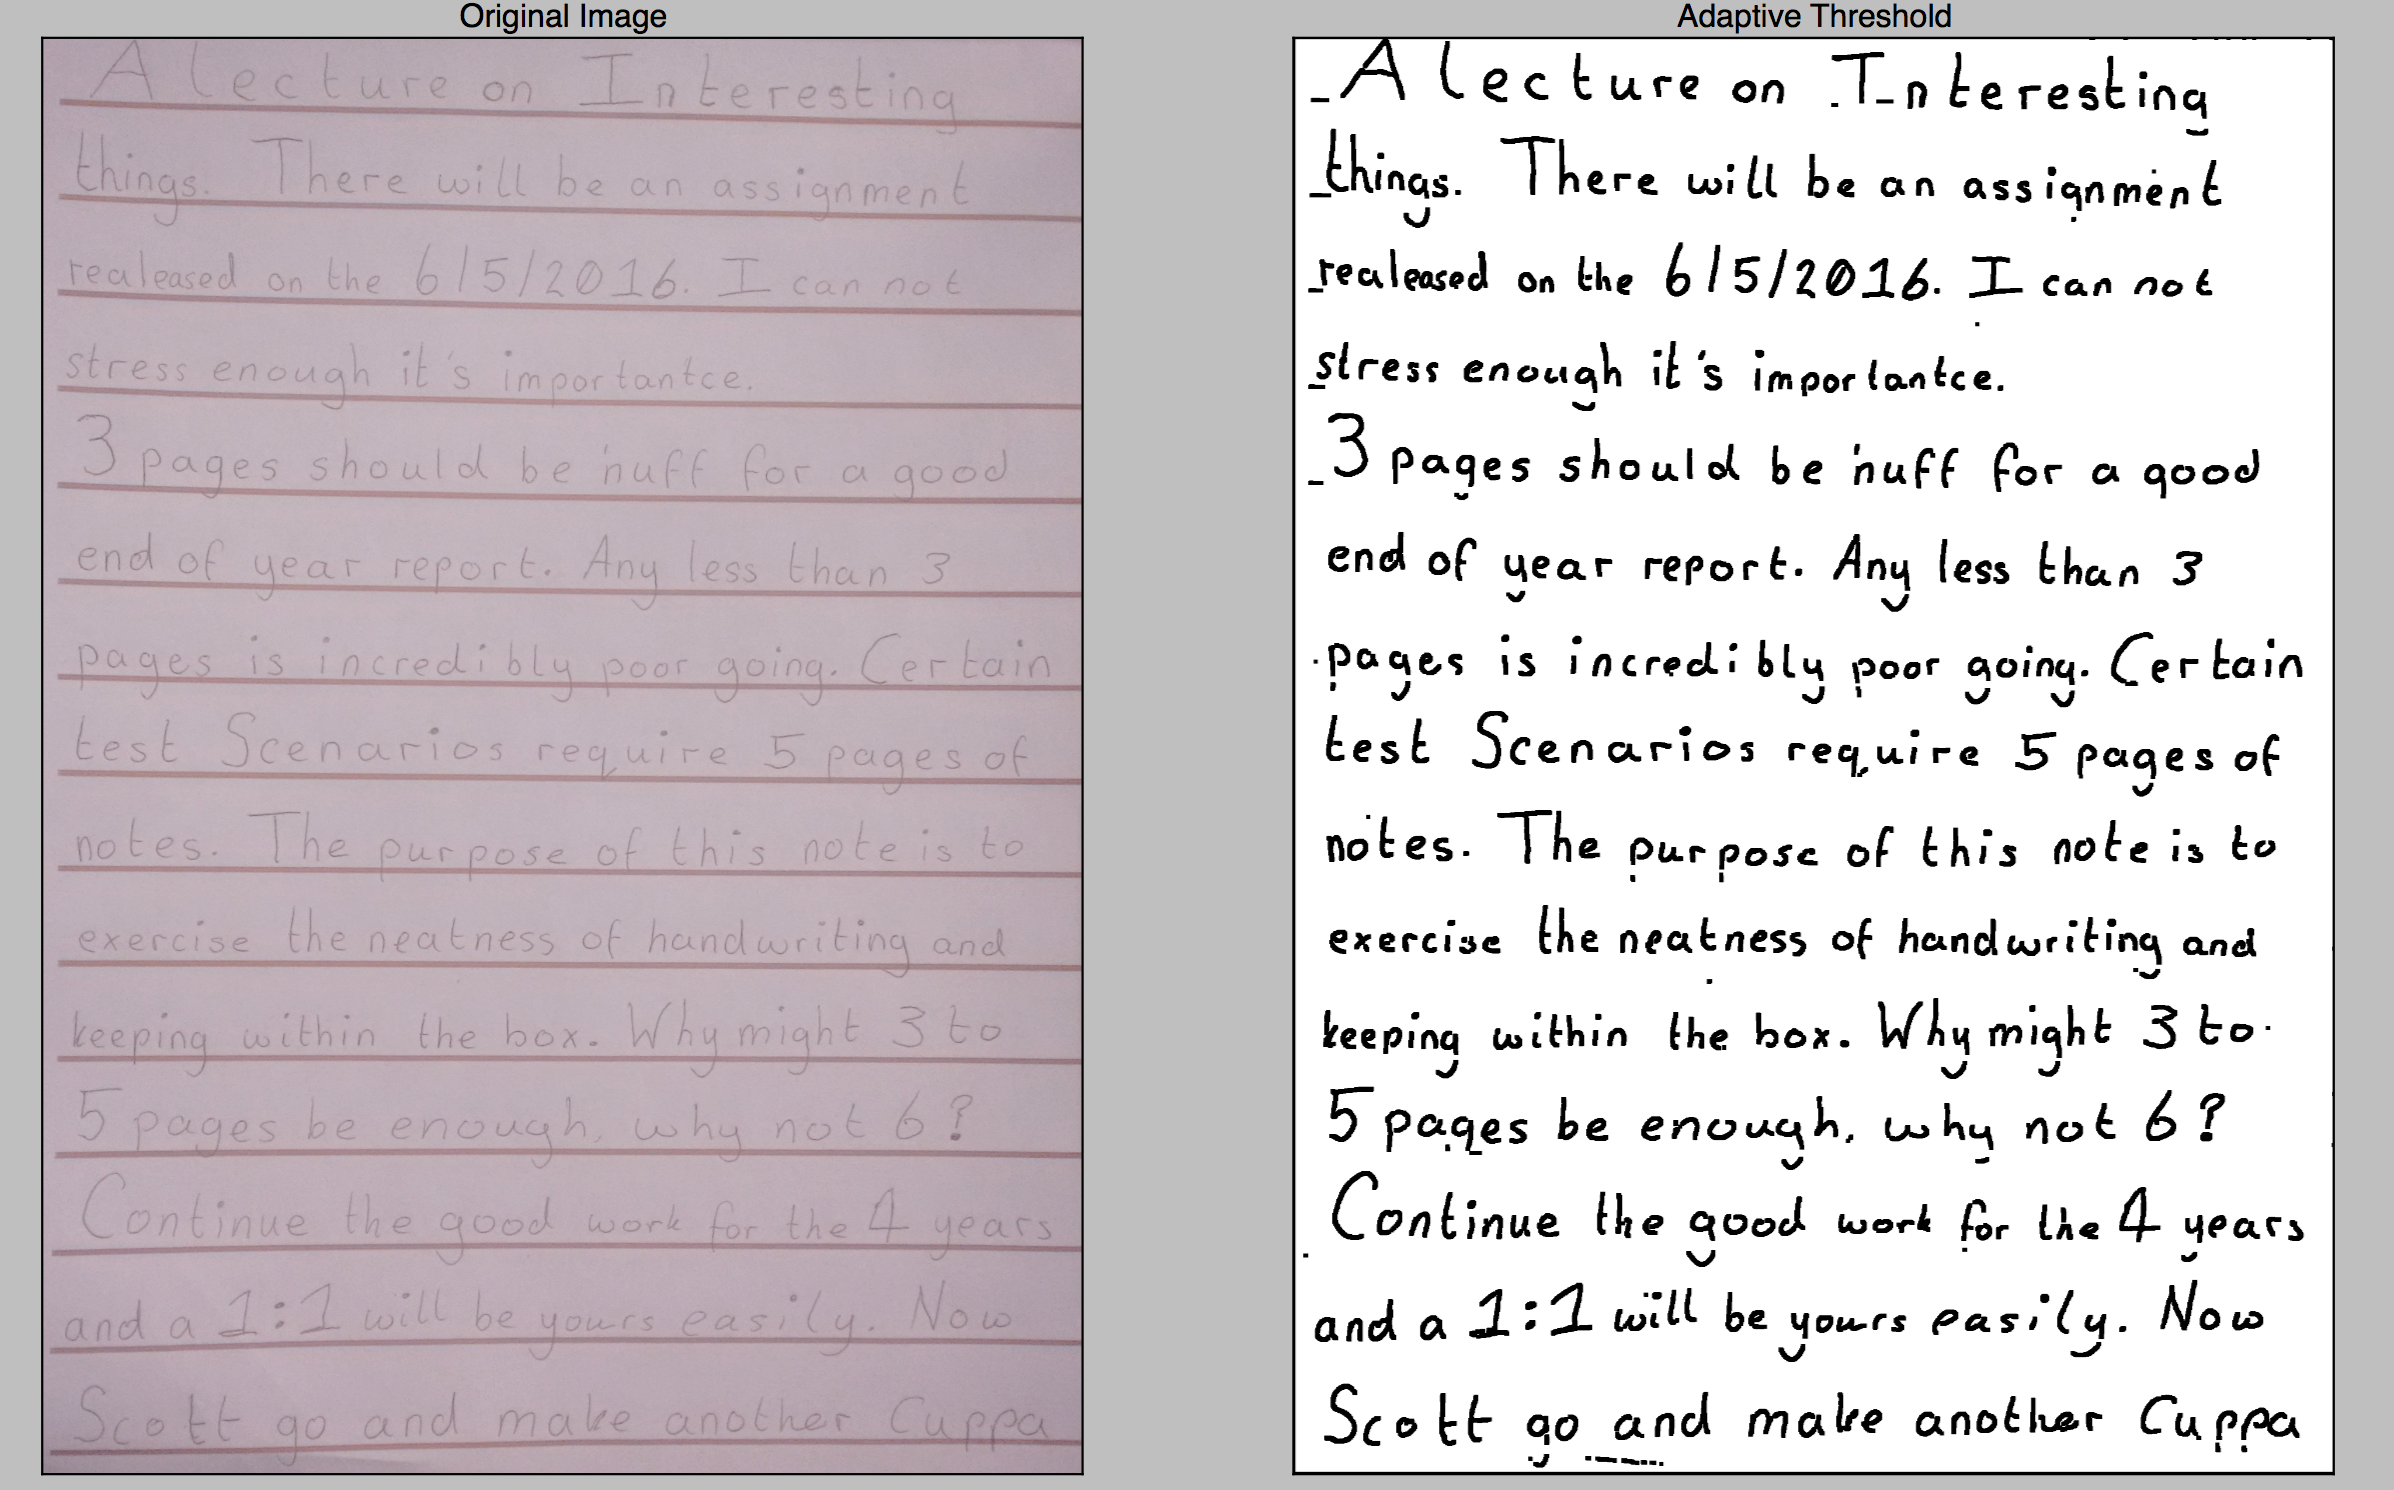
\includegraphics[scale=0.3]{images/hard_image}
  \caption{A poor quality image has been binarised successfully with little noise.}
  \label{fig:poor_quality}
\end{figure}

As shown in Figure \ref{fig:poor_quality}, the image has been successfully binarised. This shows where adaptive threshold works well - the image is a poor quality image, but it is locally thresheld. Eventually the output of the image is a clean binarisation script, with little noise. There were naturally technical difficulties along the way, and this influenced the implementation decision. Eventually it was agreed the image quality was good enough to stop the binarisation script. Further images of the iterations can be found in Appendix \ref{appendix:image_processing}.

\section{Handwriting training}
Initially the handwriting training was not yielding a good success rate. After the changes implemented from section \ref{section:threshold} the handwriting training was able to identify more characters successfully.

\subsection{Training process}
Prior to sprint 4, the training process was conducted using greyscale images. As this was not yielding much of a good recognition rate, then the binarisation script was implemented due to the problems faced.
{{\ttfamily \hyphenchar\the\font=`\-}%
Specific files formats were required during the training process with Tesseract; \texttt{<lang>.<font>.exp<number>.tiff} was the layout required for training.

When training on the test images, a selection can be found in Appendix \ref{}, Tesseract outputted a box file which contained all the characters on different lines; each lines consists of coordinates for the box file and the associated character. Initially looking at this file it was hard to identify where it was recognising characters.

\begin{figure}[H]
  \centering
  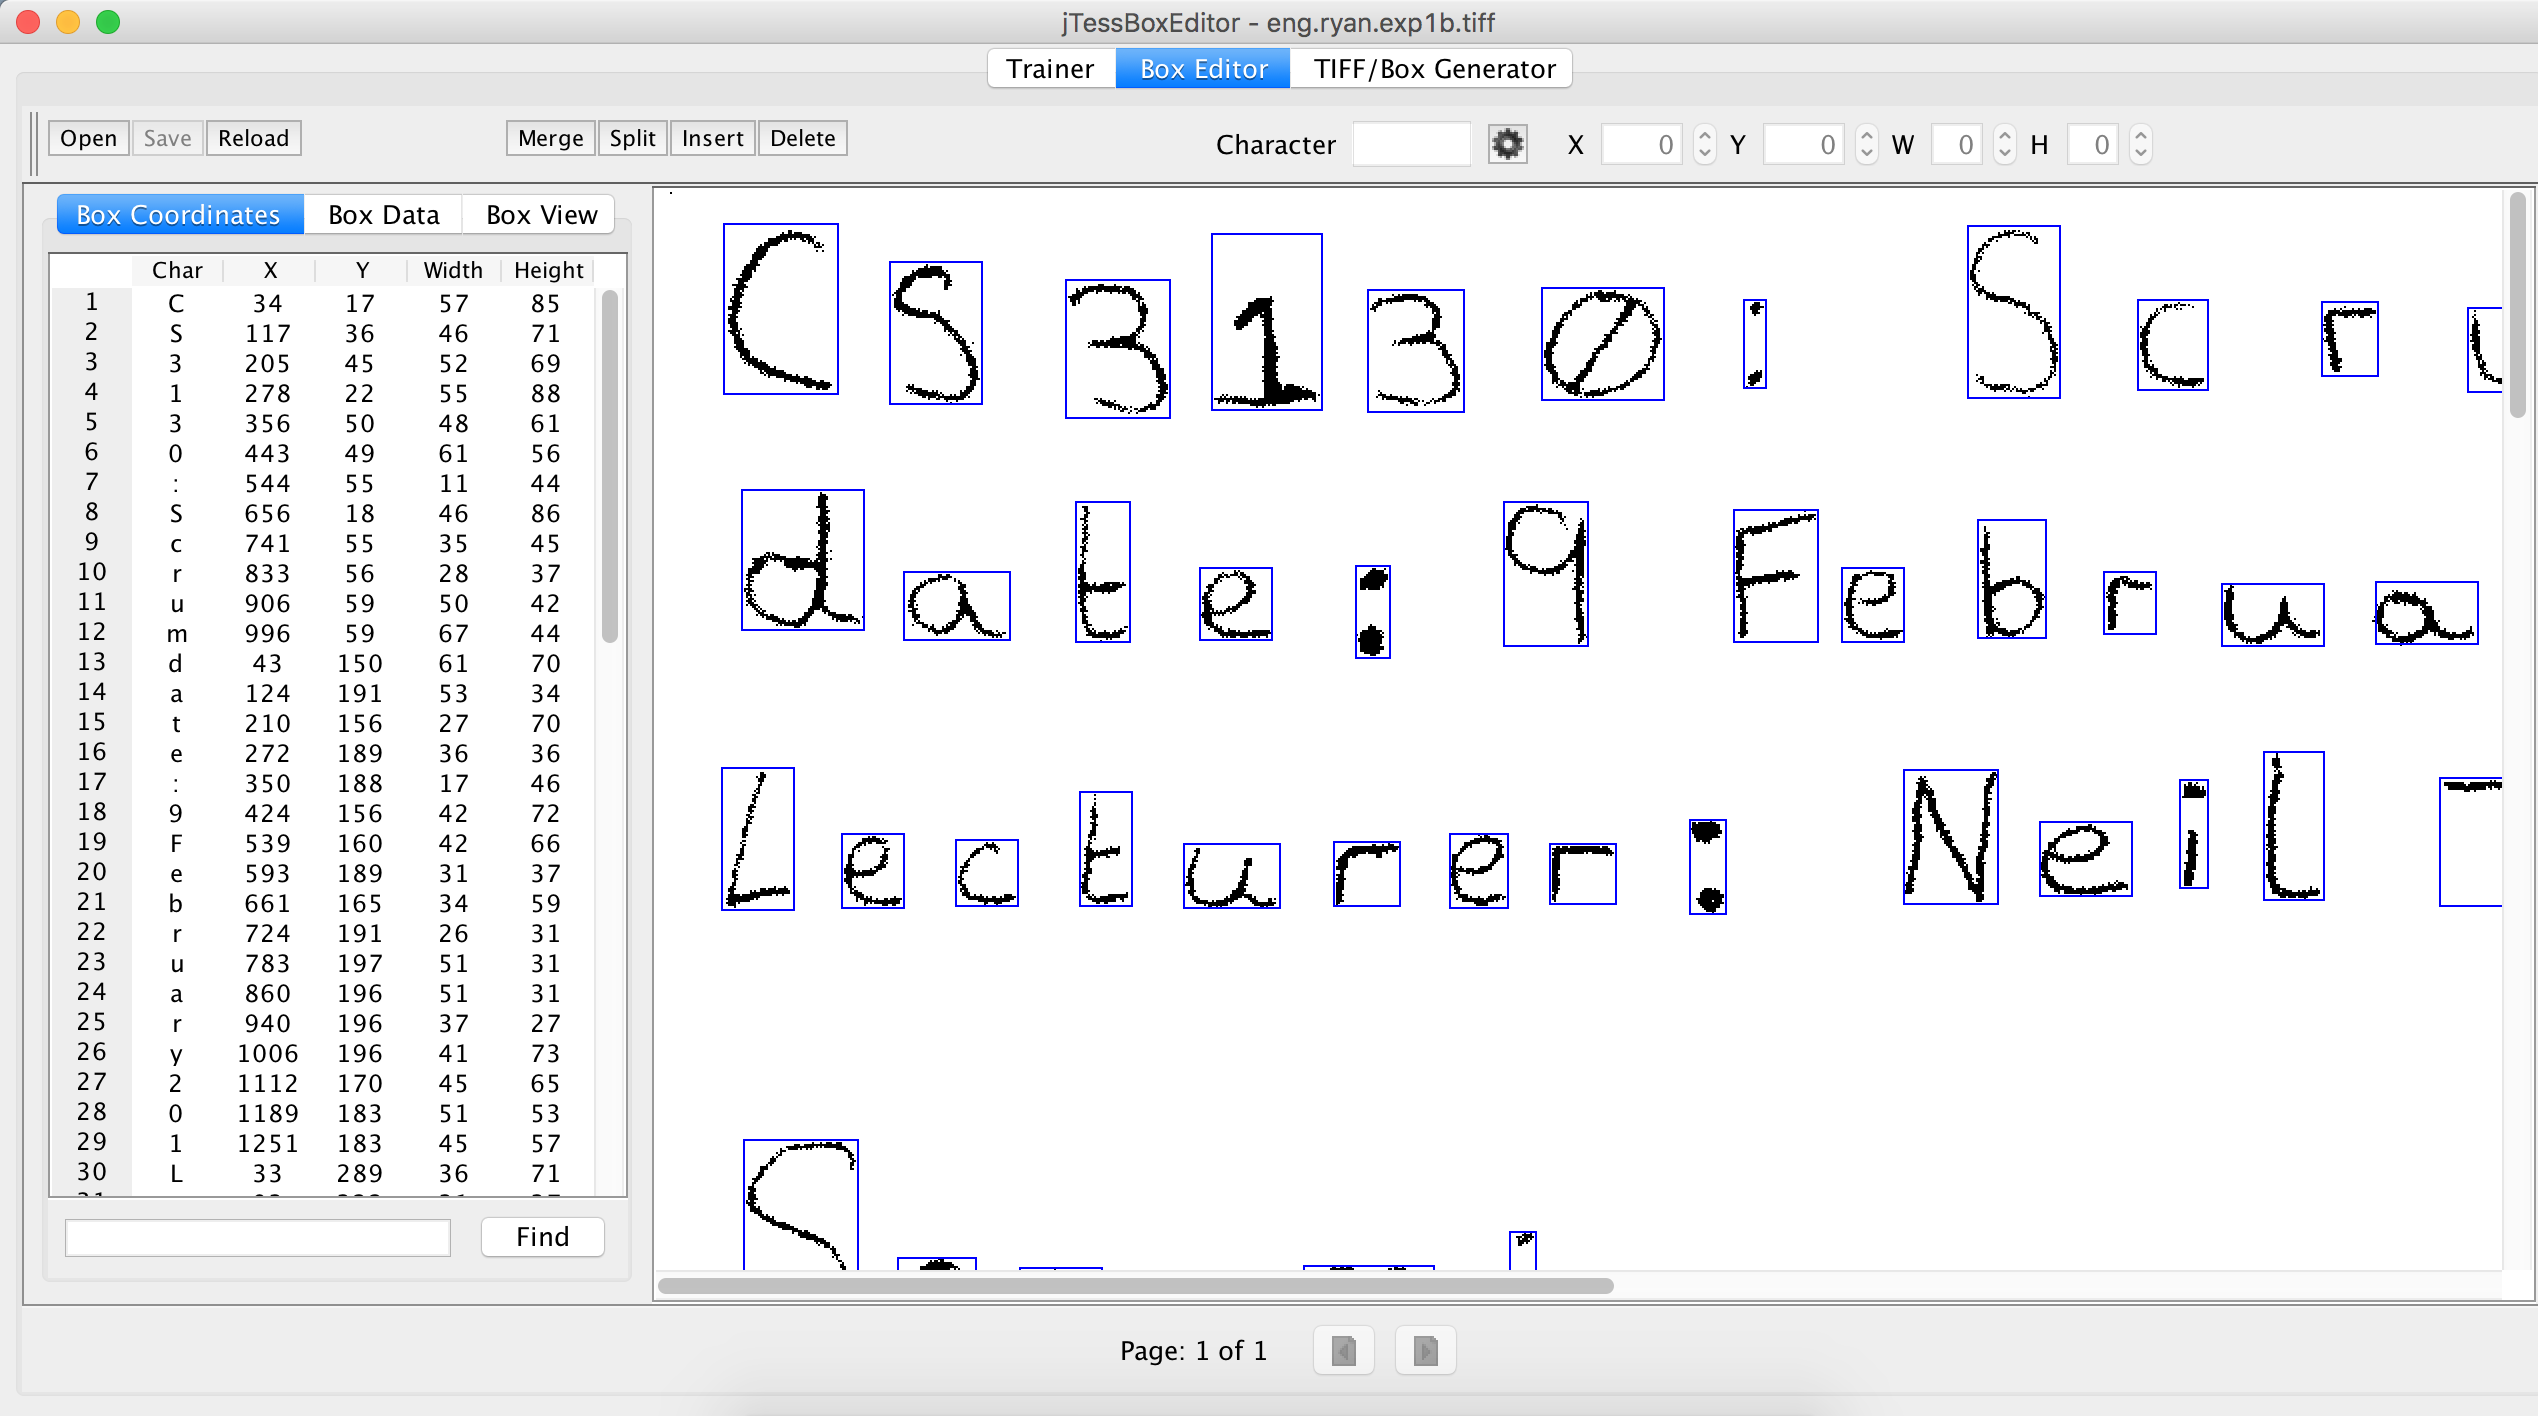
\includegraphics[width=\textwidth]{images/box_editor}
  \label{fig:box_editor}
  \caption{A example of the jTessBoxEditor being used identify characters in the tiff box file.}
\end{figure}

Figure \ref{fig:box_editor} shows the use of the tool jTessBoxEditor \cite{citeulike:13926798} when re-arranging the boxes and tagging the correct characters.

Issues were identified through the handwriting training section: sometimes characters would not be identified from the image correctly. Often when Tesseract would fail to identify a character correctly it would depict it as ``\~''. This would be split and tried to be characterised until Tesseract produced an error saying it failed to identify the characters. After a few iterations of this happening, it was decided that the best option was to remove this line from the box file.

After the tagging of characters had been completed the training process occurred. This process was repeated for each of the 12 training examples.

{{\ttfamily \hyphenchar\the\font=`\-}%
Following the guide from Github and this guys thesis:
When starting the training process, the image was trained on a new language, \texttt{eng.ryan.exp2a} along with the command \texttt{batch.nochop makebox}. This allows Tesseract to attempt to add box files, around characters which it thinks it has identified from previous examples.

{{\ttfamily \hyphenchar\the\font=`\-}%
After the identification of the characters was complete, the box file was trained using Tesseracts but in command. \texttt{tesseract <file> -l eng.ryan.exp2a box.train}. This process would attempt to train the characters for the given language. At this point there was often some errors where it can not identify the character tagged, it was learned over the itterations it was best to delete these. A trained file for the specific.

{{\ttfamily \hyphenchar\the\font=`\-}%
After training the characters, Tesseract training requires a few other files to be able to learn from the new examples. To aid in the identification of the possible characters \texttt{unicharset\_extractor} is run over all the box files. A series of characters which Tesseract can output is collated.

{{\ttfamily \hyphenchar\the\font=`\-}%
A series of clustering to ensure that characters detected could be identified again after the training process had been completed. Directed Acyclic Word Graph files were created to help to identify words and frequent word files were created to aid in improving Tesseract's chances of identifying specific characters. \texttt{/usr/share/dict/words} was piped into the words file, to ensure it had all the words in the dictionary, and additional common words such as ``by'' and ``date'' was added to the frequent words list.

{{\ttfamily \hyphenchar\the\font=`\-}%
Finally, \texttt{combine\_data} command was used to combine all the data together and output a trained data file in the form of ``eng.ryan.exp2a.trainedddata''. This was then copied to the shared Tesseract data directory resulting in a language being created for the specific user.

It is worth noting that this was done in the process a few times but it was quite lengthy, so a script was created to speed up the process. Additionally, once the language has been created once it needed to be reinforced with additional learning. This was called ``bootstrapping''. If the language was specified when learning it would reinforce that langauge and the process could start again.


\section{Web application}
The web application was the core part of the development and certain aspects proved to be more complex than others.
\subsection{OAuth}
The Google OAuth integration was a lot trickier in places than anticipated. Using the Google client library, to handle the Oauth connection reliably, was imperitive, but there was side effects from using this.

There were occassions which the Google API client raised peculiar errors; during one query it would work and then in the next query a ``rootURL'' error would be thrown. An issue was raised on the GitHub repository \cite{citeulike:14021433}. What made this issue more confusing was that it would work for querying the people plus API for the user's email address, but would constantly fail with the calendar API requests. The problem was potentially a caching issue with the application - although there was no fix for this.

During the exhanging of tokens the credentials were appended to a secure session; every page request which needed to use the credentials would select them from the session. Inside the credentials there is an expiration token, as shown in Appendix \ref{}. If this token was used to make a query then the user would be dealt with an error message, informing them they have an outdated token. As the user did not need to know about this, checks were added to ensure that the token is still valid. If it was not then it would log the user out , clearing the session, and ask them to re-authenticate.

\subsection{Reoccuring events}
Reoccurring events were to be a \textit{big} problems. Identified in the pre-beta testing, if a user had a reoccurring event then it would not append the URL to the calendar item. This design decision was not picked upon and therefore was not considered as a possibility.

All-day events were another issue. By the nature of them being all day, they do not have a date-time key in the start response from the Google Calendar API. The application would therefore error when it attempted to access a key that did not exist; this issue was resolved quickly.

The reoccuring events issues was more complex than that. When intially querying for an event, if the event was reoccurring, it would gorup the reoccurring events by their first occasion which the event was created. This proved to be problematic as it would display to the user that the note was taken on the 12th March, for example, but show an event from February.

The grouped event had a reoccurrence ID key, which was used to create another query which would return all the instances of the recocurring event; this was filtered to the start and end date of the initial query. The correct event could now be displayed.

However, when editing an reoccurring event further unexpected behaviour was experienced. After modifications to the reocurring event have been performed, and a query has been performed for all the events again, it returns both a grouped event and the instance of the edited event. So in theory it must create a new instance of an event that is reoccurring. A succinct solution was not found and instead, when parsing the events, those with the key \texttt{recurringEventId} were omitted.

\subsection{Tesseract confidence}
The Tesseract confidence went through a few iterations during the latter sprints, to achieve a better user experience.

Firstly, before any pre-processing could be implemented, the binarisation script needed to be included into the web application. It was not included until around sprint 8, where it was added as a series of function calls to the upload route. Afterwards, Tesseract was integrated into the application using tesserocr library \cite{citeulike:14021437}. A wrapper could have been written for the Tesseract's C++ API's, but due to time constraints it would not be beneficial. Figure \ref{fig:tesseract_initial} shows Tesseract originally implemented into the system.

\begin{figure}[H]
  \centering
  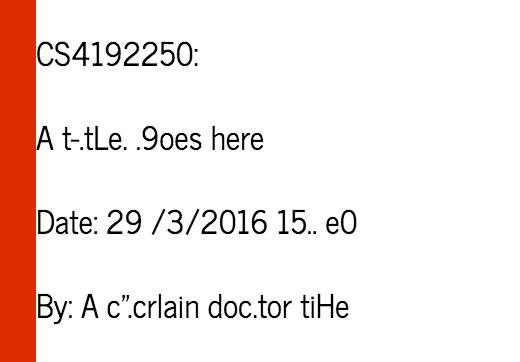
\includegraphics{images/tesseract_first}
  \label{fig:tesseract_output}
  \caption{Tesseract being integrated into the application at a very basic level}
\end{figure}

To extract the first three lines of text from an image, the tessocr library uses textlines ( an underlying feature of Tesseract), to extract all the lines which contain text in the image. Each of these lines was iterated over and all words were maped to their overall confidence.

Lines are then extracted via list-comphrension and slicing for each of the different words. A technique was tried to modify the confidence scores in the controllers, to replace the integers with the specific classname for the colours. However due to the API returning tuples, which is an immuable object, modifications could not be made easily. The eloquent envisiged would be more work than necessarily.

In the view file, checks were made on the tuple; a confidence of 75 would equate to green, less than 75 but greater than 70 would be orange and below 65 would be red. Figure \ref{fig:tesseract_colour}, shows the final coloured output. It's worth noting the anomoloy with ``Date:'', it labels it orange but it is perfectly extracted.
\begin{figure}[H]
  \centering
  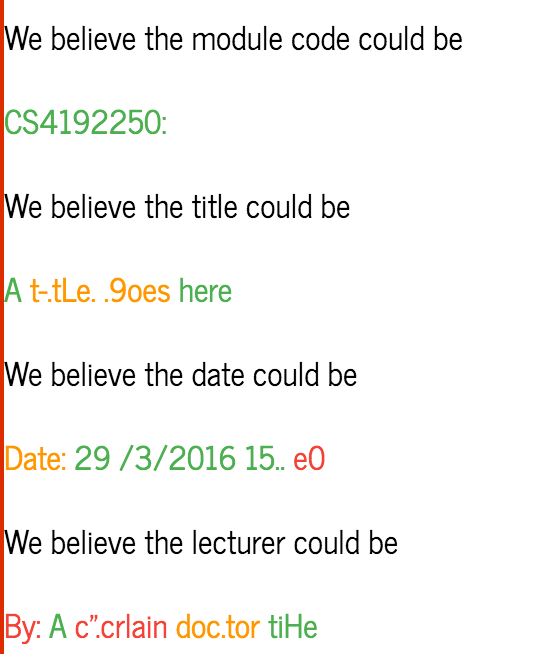
\includegraphics{images/tesseract_colour}
  \label{fig:tesseract_colour}
  \caption{Coloured representation of the confidence of the words from the handwriting.}
\end{figure}

\subsection{Parsing exif data}
One aspect of the application which was important was the parsing of exif data. Without the consideration of exif data, the initial suggestion text - which shows all the events based on a note upload - would not have been achieved.

Through the sprints, the exif data was refined and improved to allow for a greater deal of variation. Initially, Python's image library was used to get the exif data items; checks were conducted to ensure that the images were either JPEG or Tiff.

Issues arose during user-testing, when one of the participants could not upload their note probably because there was an issue with parsing EXIF data. Their mobile phone did not contain the EXIF ``dateTime'' key needed to be parsed; the key way checked to exist and the user could upload their image.

\subsection{Displaying calendar events}
Displaying the various events was adopted over several user-stories. It was first suggested by the supervisor that when a user authorises with Google it displays the last seven days on the homepage. This was fairly simple to implement, querying the Google Calendar API. What is worthy to note is that this was imperitive for integrating the other Google Services into the application - not only was it the implementation structure, but also the testing infrastructure behind it.

After parsing the exif data a story was raised to find all events based on any times found. This involved querying the external API for the events - this task was one of the first which testing began to be problematic, with mutliple requests to same service being conducted. Eventually the date was formatted from the exif time start until the end of that day at ``23:59''.

\subsection{Editing calendar events}
As discussed in the design the adding a note the user must be able to add the note URL into their calendar event. Implementing this threw a few issues. Firstly, the date was parsed by the user's input - this was then used as the query to return associated events from the Google Calendar API. Checks were then performed to ensure that the module code and the summary of the event matched.

This created the problem of being able to add to the note's URL to the correct event. If there was more than one event with the same module code that day then there could be a confusion as to which one to add to. The next itteration of the calendar events ensured that checks were made to event to validate the correct day.

An issue which was discovered was that when adding to the description field it would just replace the original content inside the description field. This is obviously a major concern as it would not allow for multiple notes per events, and it would over-write any data the user had in their description. This was changed so that it would append to the description field.

The algorithm for additng to a calendar is stated below.
\begin{algorithm}
  \caption{Adding a note URL to the calendar}
  \label{algorithm:threshold1}
  \begin{algorithmic}[1]
      \State Create a calendar service object
      \State Prepare url from saved note
      \State Build the HTTP request
      \State Find an event for that day from the start time as given
      \State Parse the events
      \State Check to see if the summary contains module code AND the start date time matches
      \If{contains module code}
        \State check the response to see if description includes url
        \State Save URL to the notes attribute in the database
      \EndIf
  \end{algorithmic}
\end{algorithm}

\begin{figure}[H]
  \centering
  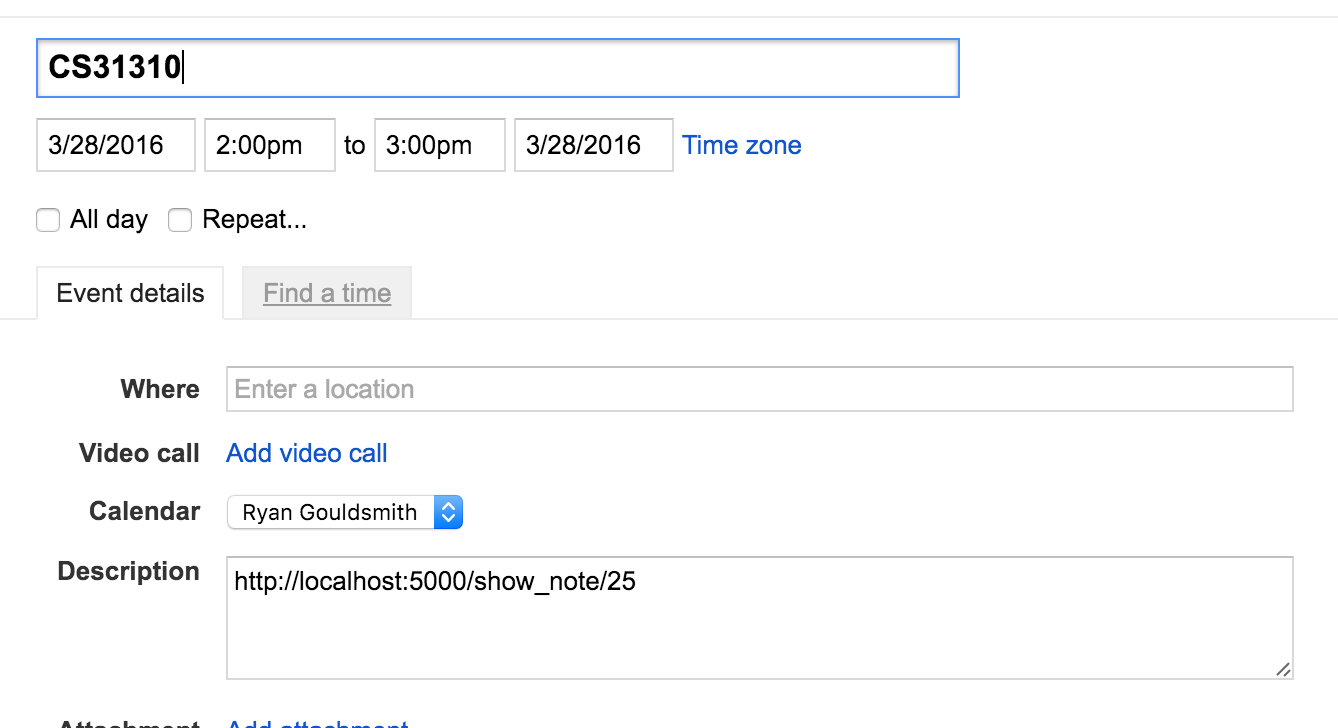
\includegraphics[scale=0.4]{images/saved_to_calendar}
  \label{fig:saved_to_calendar}
  \caption{Saving a note correctly to a calendar event item}
\end{figure}

Figure \ref{fig:saved_to_calendar} shows the output from saving a note to a specific date and it adds it to the correct calendar item.

\subsubsection{Editing a note}
During the interations it was established that when editing a note, it should reflect the changes in the user's calendar; if a user changes a date, the calendar should be updated. This design decision would prove to be a complicated implementation.

When the user edits their note, it would query the API to return the event, based on the time start which was persisted for the note. The event was intially updated in such a way it replaced the description with an empty string. This causes the problem, the same as add, where it would replace all the content. Instead, a find-and-replace on the description field, to remove the URL easily. The add was performed on the new date.

A note worth mentioning is at this point, with the editing a note, a lot of the code-base was refactored. The application was duplicating a lot of the functionality and the codebase became obfuscated. This was where the refactoring into the \texttt{GoogleServicesHelper} class was created from.

\subsubsection{Logging in and out}
Although not an original analysis decision it was decided in the design that a user's table would be implemented. When the user clicks the authorise with Google button, it uses the oAuth connection, afforementioned, and connects to the Google+ API. When connecting with the API it extracts the meta-data from the user and parses the email address, and adds it to the database.

During the sprints an issue which arose was that multiple user's were being created for a singular email address. Therefore, to reduce the problem a helper function was implemented to find existing users based on the email address. Using the SQLALchemy API's this was simplistic.

Afterwards, the user's id is appended to the user's session. This is then checked and required for every page which the user visits. When the user had finished their session, the logout route destroys everything which is in the user' sessions - forcing them to log back in again.

The decision not to use a custom-built log-in was worth it. As OAuth was being used, it was better to delegate the responsibility to a well tested system. Additionally, ethically, only an email address is being stored regarding personal information.

\section{Travis}
Although not strightly a coding implementation, Travis formed a core part of the application and was built around its successes. There were a few problems running throughout the duration of the process.

Firstly, at the start of the process time was invested to try and get the auto-deployment from Travis working correctly. Travis is able to deploy to PaaS (platform as a service) tools such as Heroku, however when trying to deploy to a custom VPS (virtual private server) issues arose. For many different attempts were conducted over several sprints to get the pipeline set up, but to no avail. Alas, Travis was used for better functionality.

Another issue, which arose when Tesseract was brought forward as a user-story, was trying to build Tesseract from source. TesserOCR, uses Tesseract 3.04 - but the latest stable package on Ubuntu is 3.02 (at the time of writing). Not only this, but Leptonia, had to be compiled from source due to Tesseract 3.04 requiring Leptonia 1.71 - and Ubuntu does not have these packages.

Additionally, this increased the build time exponentially, with building OpenCV from source as well. It now stands at around 30 minutes; caching was looked into but no solution could be found. This remains an outstanding issues.
